\section{Related Works}
\label{sec:related}

With the impressive advancements in text-to-image diffusion models~\cite{rombach2022latent}, there has been a growing interest in exploring image editing using pre-trained diffusion models. These studies have introduced several editing tasks where the user can guide the generated image through various inputs. For instance, SDEdit~\cite{meng2022sdedit} allows users to apply brush strokes to areas they wish to edit. The model then injects random noise into these targeted areas and uses the diffusion process for denoising. To create new images from examples, techniques like Textual Inversion~\cite{gal2023textual} and Dream-Booth~\cite{ruiz2023dreambooth} employ gradient-descent-based optimization to learn personalized concepts. Text-based editing, in particular, has garnered considerable interest due to its intuitive and user-friendly interaction style. In this domain, DiffusionCLIP~\cite{kim2022diffusionclip} uses DDIM inversion~\cite{song2021ddim} to reverse the diffusion process and applies fine-tuning. This approach guides the generation with a CLIP-based loss to align the generated image more closely with the intended edit.
Another method, as demonstrated in ControlNet~\cite{zhang2023adding}, involves conditioning the generation process on the edges or pose information extracted from the input image. This technique aims to generate an image that retains the original spatial structure yet {\modified{}is styled} according to the given prompt.

  \begin{figure*}[ht]
    \centering
    % import pdf
    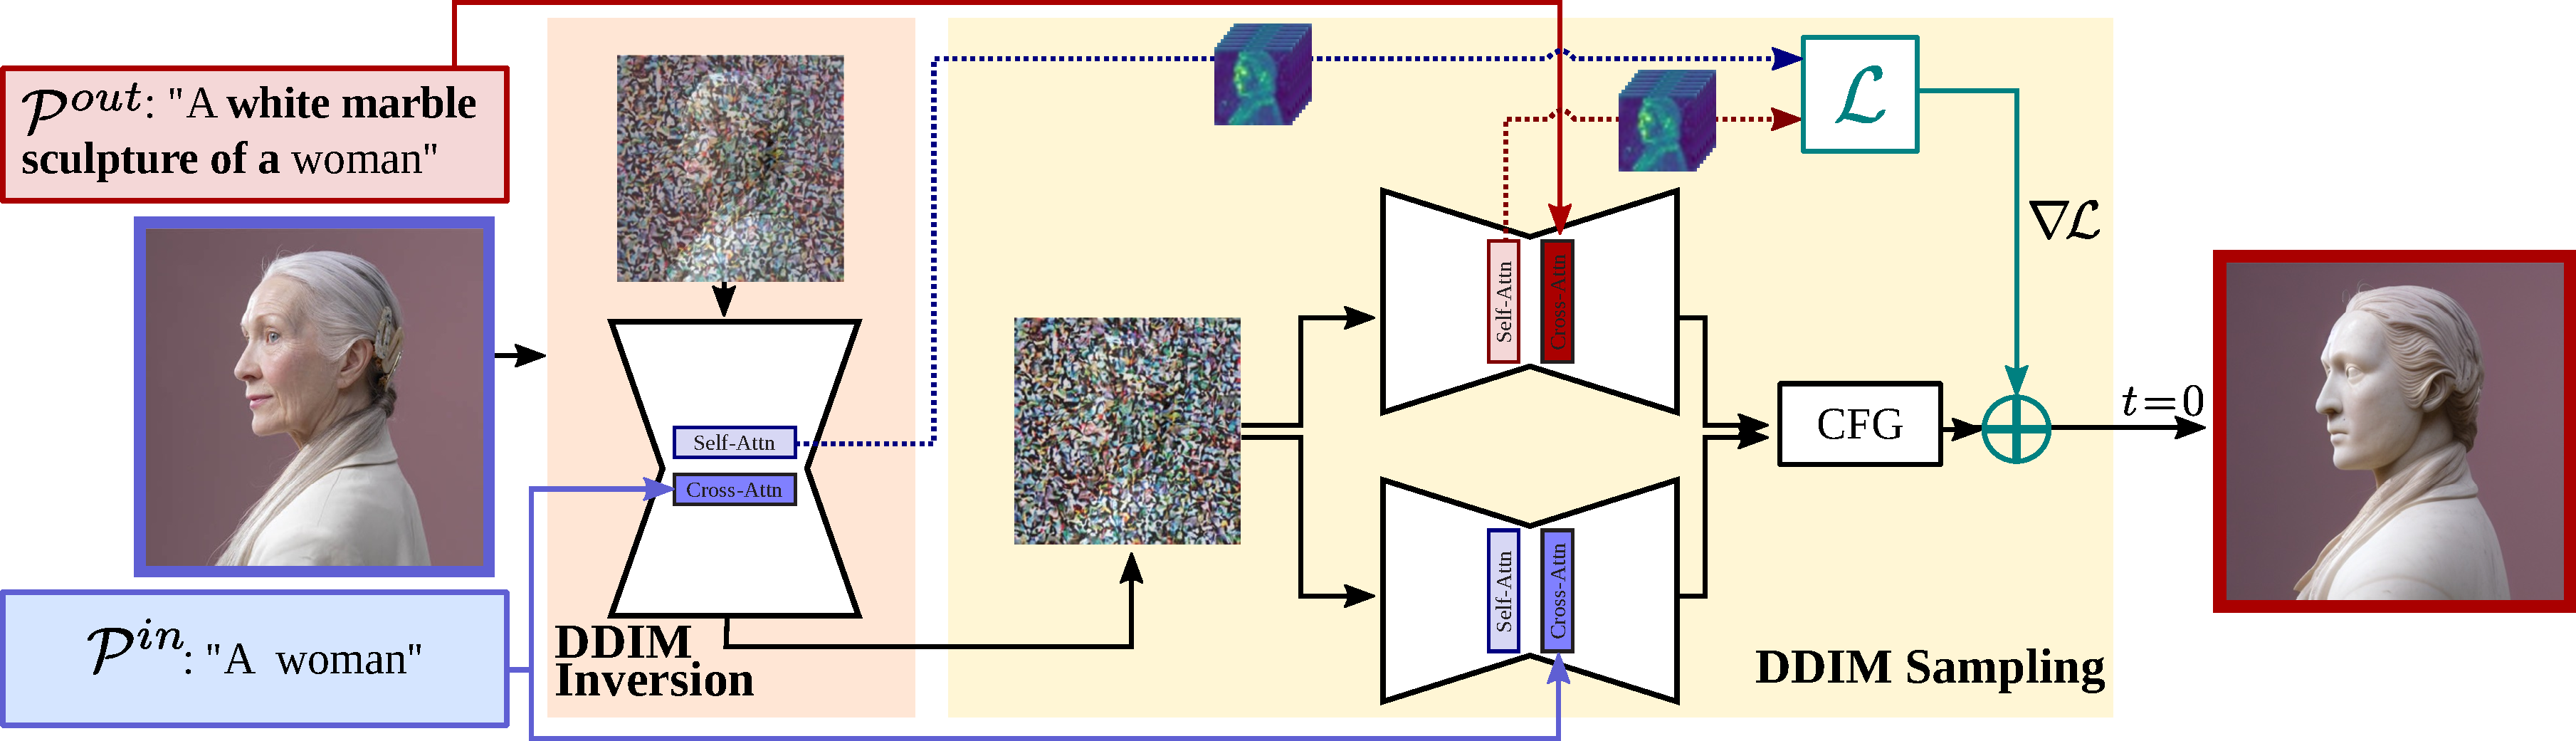
\includegraphics[width=0.85\linewidth]{fig/pipeline.pdf}
      
    \caption{
      Pipeline of \method{}: The process begins with DDIM inversion applied to the input image using its corresponding prompt, $\pin$. This inversion yields the estimated noise $\vz_T$, which serves as the initial condition for the DDIM sampling process responsible for generating the edited image. The U-Net processes both the editing prompt $\pout$ and the initial prompt $\pin$ separately, implementing classifier-free guidance. To enhance reconstruction and mitigate inaccuracies introduced by DDIM inversion, a guidance term is computed. This term is derived by comparing the self-attention maps from the DDIM inversion with those estimated by the U-Net when conditioned on the initial prompt $\pin$, ensuring closer alignment and improved fidelity in the final output.
    }
      \label{fig:method_diag}
\end{figure*}
    
{\modified{}This work focuses} on the prompt-based editing task as formulated in \cite{mokady2023null}. In this task (see Fig.~\ref{fig:teaser}) a user provides an image along with a textual prompt  $\pin$, which describes the input image. The user can then instruct the model to add, remove, change, or enhance elements in the image by providing a target prompt $\pout$ corresponding to the desired image (also called positive prompt). This problem formulation has inspired several subsequent studies~\cite{mokady2023null,parmar2023zero,tumanyan2023plug,ju2023direct}.
{\modified{}A high-level comparison is presented}  in Fig.~\ref{fig:related}, where all methods use CFG for conditioned generation and employ a mechanism to reverse the diffusion process, enabling the reconstruction of the input image from Gaussian noise. These approaches vary in their inversion mechanisms and CFG prompting strategies.

In the \nulltextlong{} (\nulltext) (see Fig.~\ref{fig:related}a), Mokady \etal{} \cite{mokady2023null} optimize the null prompt embedding fed to the diffusion model for input reconstruction, with editing facilitated via a cross-attention mechanism \cite{hertz2023prompt}. In \ptopzerolong{} \cite{parmar2023zero} (Fig.~\ref{fig:related}b), the computationally intensive inversion process is bypassed by introducing a guidance term at each diffusion step, steering the model toward accurate reconstruction. Conversely, \negativelong{} (\negative) \cite{miyake2023negative} (Fig.~\ref{fig:related}c) replaces the conventional CFG's null prompt with a negative prompt, with editing achieved through cross-attention manipulation \cite{hertz2023prompt, mokady2023null}. In \directinversionlong{} (\directinversion) \cite{ju2023direct} (Fig.~\ref{fig:related}c), the authors propose a direct inversion method that corrects the reconstruction process and introduces an edit benchmark. 
More recently, EDICT \cite{wallace2023edict} and BDIA \cite{zhang2024exact} have advanced exact diffusion inversion methods using coupled transformations and bidirectional integration approximation, respectively.

